\documentclass[12pt]{article}
%% arXiv paper template by Flip Tanedo
%% last updated: Dec 2016



%%%%%%%%%%%%%%%%%%%%%%%%%%%%%
%%%  THE USUAL PACKAGES  %%%%
%%%%%%%%%%%%%%%%%%%%%%%%%%%%%

\usepackage{amsmath}
\usepackage{amssymb}
\usepackage{amsfonts}
\usepackage{graphicx}
\usepackage{xcolor}
\usepackage{nopageno}
\usepackage{enumerate}
\usepackage{parskip}
\usepackage{framed}


\renewcommand{\thesection}{}
\renewcommand{\thesubsection}{\arabic{subsection}}

%%%%%%%%%%%%%%%%%%%%%%%%%%%%%%%%%%%%%%%%%%%%%%%
%%%  PAGE FORMATTING and (RE)NEW COMMANDS  %%%%
%%%%%%%%%%%%%%%%%%%%%%%%%%%%%%%%%%%%%%%%%%%%%%%

\usepackage[margin=2cm]{geometry}   % reasonable margins

\graphicspath{{figures/}}	        % set directory for figures

% for capitalized things
\newcommand{\acro}[1]{\textsc{\MakeLowercase{#1}}}    

%\numberwithin{equation}{section}    % set equation numbering
\renewcommand{\tilde}{\widetilde}   % tilde over characters
\renewcommand{\vec}[1]{\mathbf{#1}} % vectors are boldface

% \newcommand{\dbar}{d\mkern-6mu\mathchar'26}    % for d/2pi
\newcommand{\dbar}{d\mkern-6mu\mathchar'26\hspace{-.1em}}    % spacing
\newcommand{\ket}[1]{\left|#1\right\rangle}    % <#1|
\newcommand{\bra}[1]{\left\langle#1\right|}    % |#1>
\newcommand{\Xmark}{\text{\sffamily X}}        % cross out

\let\olditemize\itemize
\renewcommand{\itemize}{
  \olditemize
  \setlength{\itemsep}{1pt}
  \setlength{\parskip}{0pt}
  \setlength{\parsep}{0pt}
}


% Commands for temporary comments
\newcommand{\comment}[2]{\textcolor{red}{[\textbf{#1} #2]}}
\newcommand{\flip}[1]{{\color{red} [\textbf{Flip}: {#1}]}}
\newcommand{\email}[1]{\texttt{\href{mailto:#1}{#1}}}

\newenvironment{institutions}[1][2em]{\begin{list}{}{\setlength\leftmargin{#1}\setlength\rightmargin{#1}}\item[]}{\end{list}}


\usepackage{fancyhdr}		% to put preprint number



% Commands for listings package
%\usepackage{listings}      % \begin{lstlisting}, for code
%
% \lstset{basicstyle=\ttfamily\footnotesize,breaklines=true}
%    sets style to small true-type



%%%%%%%%%%%%%%%%%%%
%%%  HYPERREF  %%%%
%%%%%%%%%%%%%%%%%%%

%% This package has to be at the end; can lead to conflicts
\usepackage{microtype}
\usepackage[
	colorlinks=true,
	citecolor=black,
	linkcolor=black,
	urlcolor=green!50!black,
	hypertexnames=false]{hyperref}





\begin{document}


\begin{center}

    {\Large \textsc{Long HW 2}:
    \textbf{Indices. Indices everywhere.}}
    
\end{center}

\vskip .4cm

\noindent
\begin{tabular*}{\textwidth}{rl}
	\textsc{Course:}& Physics 165, \emph{Introduction to Particle Physics} (2020)
	\\
	\textsc{Instructor:}& Prof. Flip Tanedo (\email{flip.tanedo@ucr.edu})
	\\
	\textsc{Due by:}& {Thursday}, April 28
\end{tabular*}

\noindent
This is the main 2-week homework set. Unless otherwise stated, give all responses in natural units where $c = \hbar = 1$ and energy is measured in electron volts (usually MeV or GeV). 


\subsection{Two-Body Phase Space}
[ This problem is inspired by a problem in Larkoski's text, chapter 4. ] The cross section for a scattering process includes an integral over \emph{phase space}: the possible kinematics (four-momenta) of the final state particles. If we are too naive, then we would say that the phase space is simply an integral over all possible 4-momenta for each final state. Thus if the final state has $n$ particles, we would naively say that the phase space $\Pi_n$ is
\begin{align}
	\int d\Pi_n \stackrel{?}{=} \int \prod_{i=1}^n \dbar^4 p_i \ ,
\end{align}
where $\dbar = d/(2\pi)$. This is wrong. One reason why it is wrong is that the final state particles need to be on-shell. This means that $p_i^2 = E_i^2 - \vec{p}_i^2 = m_i^2$. We can impose on-shell-ness by sticking on a $\delta$-function to the phase space:
\begin{align}
	\int d\Pi_n \stackrel{?}{=} \int \prod_{i=1}^n \dbar^4 p_i\, (2\pi)\delta(p_i^2 - m_i^2) \ .
\end{align}
The factors of $(2\pi)$ come from our conventions for $\delta$-functions and Fourier transforms. There is nothing deep about them, so we will not make a big deal about these prefactors.
It turns out that our phase space is \emph{still} too naive. We need to impose total four-momentum conservation. Let $Q^\mu$ be the total four-momentum of the inital state. Then we can stick on an additional overall four-momentum conserving $\delta$-function: 
\begin{align}
	\int d\Pi_n {=} \int (2\pi)^4 \delta^{(4)}\left(Q-\sum_i^N p_i\right) \prod_{i=1}^n \dbar^4 p_i\, (2\pi)\delta(p_i^2 - m_i^2) \ .
\end{align}
Again, we won't make a big deal about the factors of $(2\pi)$. Note that the factors are each manifestly Lorentz invariant.


In this problem we will use this expression to determine the phase space for a process with two final state particles,
\begin{align}
	\int d\Pi_2 {=} 
	\int (2\pi)^4 \delta^{(4)}\left(Q-p_1-p_2\right) 
	\;
	\dbar^4 p_1\, (2\pi)\delta(p_1^2 - m_1^2) 
	\;
	\dbar^4 p_2\, (2\pi)\delta(p_2^2 - m_2^2)
	\ .
\end{align}
Here $p_1$ and $p_2$ are the four-momenta of the two final state particles of masses $m_1$ and $m_2$.

\subsubsection{Integration over on-shell conditions}

Perform the integration over the two on-shell conditions with respect to the energies of the final state momenta, $dp_1^0$ and $dp_2^0$.  You should end up with
\begin{align}
	\int d\Pi_2 = 
	\int \frac{\dbar^3 \vec{p}_1}{2E_1} \, \frac{\dbar^3 \vec{p}_2}{2E_2}
	\;
	(2\pi)^4 \delta^{(4)}(Q-p_1-p_2) \ .
\end{align}
At this point, the final state energies $E_1$ and $E_2$ are functions of the three-momenta. For example, $E_1(\vec{p_1}) = m_1^2 + \vec{p}_1^2$.


\textsc{Hint:} it may be helpful to recall the relation
\begin{align}
	% \delta(y-f(x)) = \sum_{x_i} \left.\frac{\delta(x-x_i)}{|df/dx|}\right|_{f(x_i)=0} \ .
	\delta(y-f(x)) = \frac{\delta(x-f^{-1}(y))}{|df/dx|} \ .
\end{align}

\subsubsection{Center of momentum frame}

Now assume that you are in the center of momentum frame for the initial state. This means that the total four-momentum is simply
\begin{align}
	Q = \left(E_\text{CM}, 0, 0, 0\right) \ .
\end{align}
Use the total four-momentum conserving $\delta$-function to integrate over the three-momentum of the second final state particle, $\dbar \vec{p}_2$. It should be easy to find that
\begin{align}
	\int d\Pi_2 = \int \frac{\dbar^3\vec{p}_1}{2E_1\, 2E_2} \;
	(2\pi)\delta(E_\text{CM} - E_1 - E_2) \ .
\end{align}

\subsubsection{Spherical Coordinates}

Pass to spherical coordinates for $\vec{p}_1$. Note that the energies are independent of the angular coordinates. They do, however, depend on the magnitude $|\vec{p}_1| = |\vec{p}_2| \equiv p$. Integrate over the remaining $\delta$-function to show that
\begin{align}
	\int d\Pi_2 = \frac{1}{16\pi^2}\frac{p}{E_\text{CM}} \int_0^{2\pi} d\phi \int_{-1}^1 d\cos\theta \ .
\end{align}

\textsc{Comment:} the phase space integration has other terms, including the squared amplitude, that typically depend an angle of one of the final state particles relative to one of the initial state particles. It is convenient to align the $\vec{p}_1$ axes along the initial state axis so that $\cos\theta$ encodes this angular dependence. On the other hand, the squared amplitude does not depend on the azimuthal angle $d\phi$ and this integral just gives a factor of $(2\pi)$.




% \subsection{Momentum In a Loop}

% Here's a diagram for a higher-order correction to $e^+ e^- \to Z$. 
% \begin{center}
% 	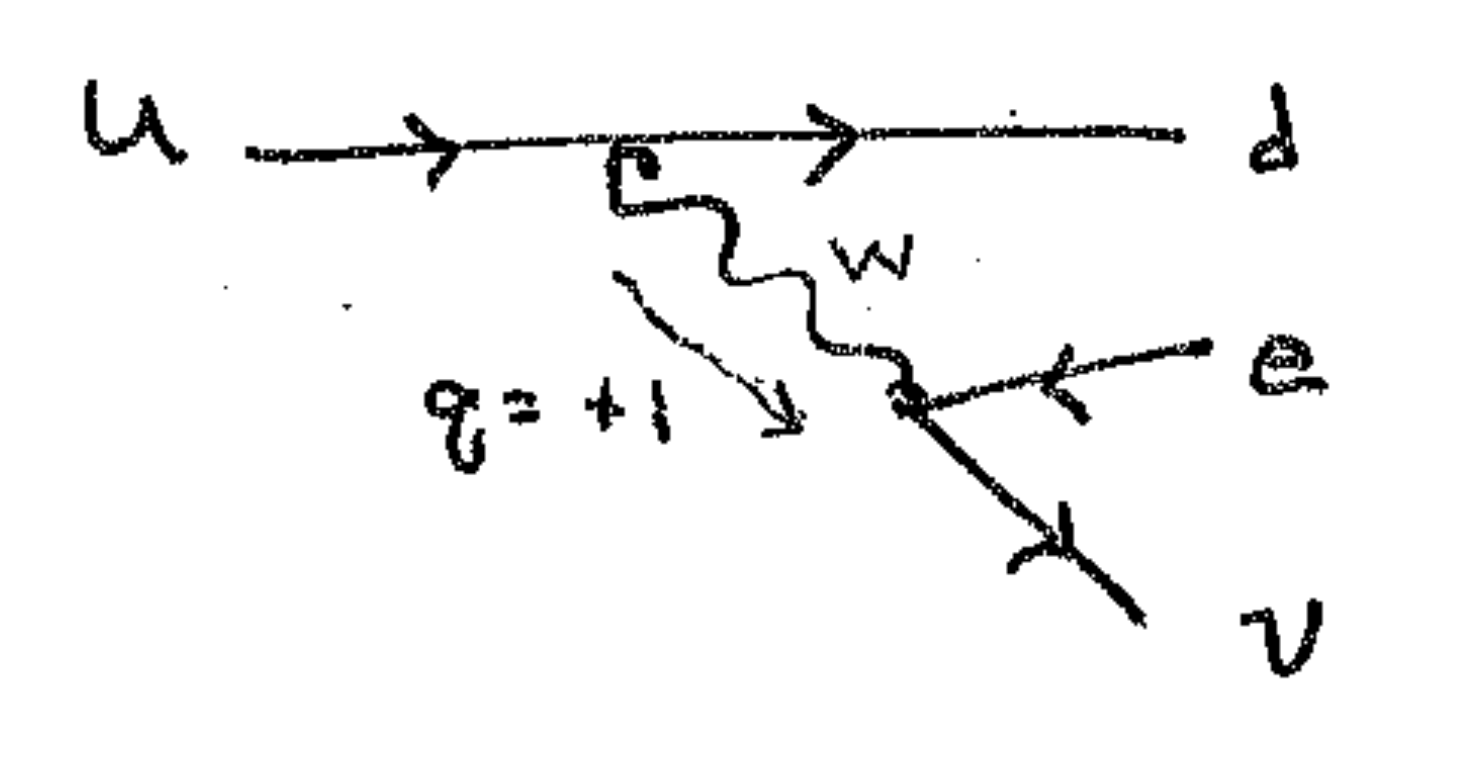
\includegraphics[width=.4\textwidth]{HW2b.png}
% \end{center}

% \subsubsection{What are the internal lines?}

% In the diagram above, what are the possible particle species of the internal lines? Label them. Choose from $e,\mu, \nu_e, \nu_\mu, \gamma, Z$. 

% \subsubsection{In-state/out-state kinematics}

% In the center of mass frame for the system (the rest frame of the $Z$), what condition must be satisfied by the electron and positron momenta for this process to be kinematically possible? Now write this in terms of an \emph{invariant} quantity of the $e^+e^-$ system, so that you can specify a condition which must be true in \emph{any} frame.

% \textsc{Discussion}: The remarkable observation about this process is that it looks like you need to tune your electron--positron energies to be \emph{exactly} the right in order to produce the $Z$ boson on-shell. This is in contrast to $e^+e^- \to \mu^+ \mu^-$, where as long as you have enough energy, you can produce the muons. If your $e^+e^-$ system has a little extra energy, then the muons are a little more energetic. In $e^+e^- \to Z$, if you give your $e^+e^-$ system a little extra energy, then you cannot produce the $Z$ on-shell. We will see that there's a little more to this story than we're presenting.

% \subsubsection{Loop momentum}

% Use conservation of four-momentum at each vertex to determine $q_1^\mu$, $q_2^\mu$ and $q_3^\mu$ in terms of the observed four-momenta, $p_1^\mu$, $p_2^\mu$, and $k_1^\mu$. 

% \subsubsection{That's weird...}

% In the previous sub-problem, you should find that you cannot determine $q_{1,2,3}$ uniquely. What do you think this means in terms of the sum of amplitudes? Think about it this way: each possible assignment of momentum flow is a possible history between the $|\text{ in }\rangle$ and the $|\text{ out }\rangle$ states. Answer in a few sentences. 

% \textsc{Comment}: There's no strict criteria for what you must answer, but I'd like you to think about this and convey (i) understanding of the situation and (ii) thoughts/speculation about interpretation.



\subsection{Indices and what they tell us}

The ``index-ology'' that we're proposing has a high-brow name: the representation theory of Lie groups. We will use the Define the \textbf{Einstein summation convention}:
\begin{quote}
	Repeated indices are summed over. 
\end{quote}
 There's no physics and no mathematics in this, it's simply a shorthand to avoid writing the sum symbol. \emph{Most of the time} we require that one of the repeated indices is upper and the other is lower. In this problem that is indeed the case. Thus, for example:
 \begin{align}
 	T^{i}_{\phantom{i}j}y^j \equiv \sum_j T^{i}_{\phantom{i}j}y^j = T^{i}_{\phantom{i}1}j^1 + T^{i}_{\phantom{i}2}y^2 + \cdots \ .
 \end{align}
 This object has one \textbf{free index}, $i$, because the $j$ index is repeated and hence summed over. In other words: in order to get a \emph{number}, I have to specify what $i$ is. 


\subsubsection{Rotations: SO(2)}

SO(2) is the fancy name for rotations in two-dimensional space. Let's introduce two kinds of objects that transform under rotations: \textbf{column vectors}, $v^i$, and \textbf{row vectors}, $w_j$.% You could also call these $\vec{v}$ and $\vec{w}^T$.

\begin{framed}
\textsc{Caveats!} I am now guilty of propagating some terrible misunderstandings that are unfortunately rife among physics students. Here are some of them:
\begin{enumerate}
	\item There are many words for the objects that I'm calling column and row vectors. The words that we're using should be the most familiar, but it's also the notation that mathematicians use for their kindergarten-age children. If you're ever in a cocktail party with mathematicians, then you might want to say things like covariant/contravariant, or vector/one-form, or vector/dual vector. These sound way fancier, but for our immediate purposes do not convey any deeper meaning. 
	\item Much worse, I'm voluntarily committing the cardinal sin of using the \emph{components} of an object to represent the object itself. I'm assuming that we have all agreed upon the right basis $\vec{e}_{(1)}$ and $\vec{e}_{(2)}$, so that writing $v^i$ can mean either vector $$\vec{v} = v^1 \vec{e}_{(1)} + v^2 \vec{e}_{(2)},$$ or the $i^\text{th}$ component of that vector, that is $v^1$ for $i=1$ or $v^2$ for $i=2$. The basis vectors are abstract objects and don't have to represent anything; but they could be, for example, any of the following:
\begin{align}
	\vec{e}_{(1)} & = \begin{pmatrix}1\\0\end{pmatrix}
	&
	\vec{e}_{(2)} & = \begin{pmatrix}0\\1\end{pmatrix}
	\\
	\vec{e}_{(1)} & = \frac{1}{\sqrt{2}}\begin{pmatrix}0\\1\\1\end{pmatrix}
	&
	\vec{e}_{(2)} & = \frac{1}{\sqrt{2}}\begin{pmatrix}0\\1\\-1\end{pmatrix}
	\\
	\vec{e}_{(1)} & = \left|\text{ cat alive } \right\rangle
	&
	\vec{e}_{(2)} & = \left|\text{ cat dead } \right\rangle
\end{align}
or any other orthonormal set of objects. The point is that we've agreed upon what they are (or agreed to not worry about it) and that we'll focus on the components $v^1$ and $v^2$.
\end{enumerate}
\end{framed}
Here are the rules for upper and lower indices:
\begin{enumerate}
	\item Each upper index transforms with a rotation matrix, $R^i_{\phantom i j}$. 
	\item Each lower index transforms with a rotation matrix in the opposite direction, $(R^{-1})^i_{\phantom i j}$. 
\end{enumerate}
thus we have the transformation rules that under a rotation by $\theta$,
\begin{align}
	v^i &\to (v')^i = R^i_{\phantom i j} v^j = R^i_{\phantom i 1}v^1 + R^i_{\phantom i 2}v^2
	\label{eq:v}
	\\
	w_j &\to (w')_j = (R^{-1})^i_{\phantom i j} w_i = (R^{-1})^1_{\phantom 1 j}w_1 + (R^{-1})^2_{\phantom 2 j}w_2 \ .
	\label{eq:w}
\end{align}
The components of a rotation are:
\begin{align}
	R^1_{\phantom 1 1} &= \cos \theta
	&
	R^1_{\phantom 1 2} &= \sin\theta
	&
	R^2_{\phantom 2 1} &= -\sin\theta
	&
	R^2_{\phantom 2 2} &= \cos \theta 
	\label{eq:rot}
	\\
	(R^{-1})^1_{\phantom 1 1} &= \cos \theta
	&
	(R^{-1})^1_{\phantom 1 2} &= -\sin\theta
	&
	(R^{-1})^2_{\phantom 2 1} &= \sin\theta
	&
	(R^{-1})^2_{\phantom 2 2} &= \cos \theta \ .
\end{align}

Explicitly write the components $(v')^i$ and $(w')_j$ in terms of the components $v^i$ and $w_j$. For example, the first one is:
\begin{align}
	(v')^1 = \cos \theta \, v^1 + \sin\theta  \, v^2 \ .
\end{align}
Confirm that this is indeed the same thing as ordinary matrix multiplication,
\begin{align}
\vec{v}' &=
 \begin{pmatrix}
		\cos \theta & \sin \theta \\
		-\sin \theta & \cos \theta
	\end{pmatrix}
	\begin{pmatrix}
		v^1 \\
		v^2
	\end{pmatrix} 
	&
\vec{w'}^T &=
\left[
 \begin{pmatrix}
		\cos \theta & \sin \theta \\
		-\sin \theta & \cos \theta
	\end{pmatrix}
	\begin{pmatrix}
		w^1 \\
		w^2
	\end{pmatrix} \right]^T
	\ .
\end{align}

\textsc{Remark}: yes, you \emph{know} what the answer is---do it using the sums in (\ref{eq:v}) and (\ref{eq:w}) so that you see how the notation works.

\subsubsection{How matrices transform} 

The object that you know of as a `matrix' has one upper and one lower index. Each index transforms according to the rules above:
\begin{align}
	M^i_{\phantom i j} 
	\to (M')^i_{\phantom{i} j} 
	= (R^{-1})^k_{\phantom{k} j} R^i_{\phantom{i}\ell} M^\ell_{\phantom\ell k} \ .
\end{align}
Confirm that this is equivalent to the `usual' rule
\begin{align}
	\begin{pmatrix}
		m^1_{\phantom 1 1} & m^1_{\phantom 1 2}
		\\
		m^2_{\phantom 2 1} & m^2_{\phantom 2 2}
	\end{pmatrix}
	\to 
	\begin{pmatrix}
		\cos \theta & \sin \theta \\
		-\sin \theta & \cos \theta
	\end{pmatrix}
	\begin{pmatrix}
		m^1_{\phantom 1 1} & m^1_{\phantom 1 2}
		\\
		m^2_{\phantom 2 1} & m^2_{\phantom 2 2}
	\end{pmatrix}
	\begin{pmatrix}
		\cos \theta & -\sin \theta \\
		\sin \theta & \cos \theta
	\end{pmatrix} \ .
	\label{eq:rotation:matrix}
\end{align}

\textsc{Remark}: Observe that unlike the usual matrix multiplication where the order of the matrices matter, 
\begin{align*}
(R^{-1})^k_{\phantom{k} j} R^i_{\phantom{i}\ell} M^\ell_{\phantom\ell k}
=
(R^{-1})^k_{\phantom{k} j}  M^\ell_{\phantom\ell k}	R^i_{\phantom{i}\ell}
=
R^i_{\phantom{i}\ell}  M^\ell_{\phantom\ell k} (R^{-1})^k_{\phantom{k} j}
= \cdots
\end{align*}
This is because the summation convention is taking care of the  kindergarten matrix multiplication rule that one should `tip the matrix over and then sum the pieces that hit the next matrix.' More importantly, this lets us generalize that rule to the case of objects with many indices. 

\subsubsection{An SO(2) invariant} 

We say that objects with indices are \textbf{covariant}, they change in a specific way with respect to rotations. This is in contrast to objects with no indices, which are \textbf{invariant} or \textbf{scalar}. 

Because $v^i$ has an upper index an $w_j$ has a lower index, you can \textbf{contract} them to form an object with no indices:
\begin{align}
	v^i w_i \equiv v^1 w_1 + v^2 w_2  \ .
\end{align}

Confirm that this object---which you know as the usual dot product---is indeed invariant by calculating $(v')^i(w')_i$. 

\subsubsection{The metric on flat two-dimensional space} 

We can introduce an additional mathematical structure to our vector space: a \textbf{metric}. This is an object that lets us raise and lower indices. In 2D flat space, we know this operation as \textbf{transpose}. More generally, it is the Kronecker $\delta$:
\begin{align}
	\delta_{ij} &=
	\left\{
	\begin{array}{lcl}
		1 & \quad & \text{if $i = j$}\\
		0 & \quad & \text{otherwise}
	\end{array}
	\right.
	&
	\delta^{ij} &=
	\left\{
	\begin{array}{lcl}
		1 & \quad & \text{if $i = j$}\\
		0 & \quad & \text{otherwise}
	\end{array}
	\right.
\end{align}
Thus we may write
\begin{align}
	v\cdot v = v^i v_i = v^i (\delta_{k i} v^k) \ ,
\end{align}
where in the last equation we have used the $\delta_{ki}$ to create a lower-index object $v_i$ out of an upper-index object, $v^k$. This lets us define a \textbf{norm} of a vector:
\begin{align}
	|\vec v| = \sqrt{v\cdot v} \equiv \sqrt{ \delta_{k i} v^iv^k} \ .
\end{align}
Confirm the trivial statement that the lower-index $\delta_{ij}$ is the \emph{inverse} of the upper-index $\delta^{ij}$. In other words, confirm that
\begin{align}
	\delta_{ik}\delta^{kj} = \delta_i^j &=
	\left\{
	\begin{array}{lcl}
		1 & \quad & \text{if $i = j$}\\
		0 & \quad & \text{otherwise}
	\end{array}
	\right. \ .
\end{align}

\subsubsection{Boosts: SO(1,1)}

SO(1,1) is the fancy name for Lorentz transformations in two-dimensional space\emph{time}. To distinguish from just space, we will use lowercase Greek letters like $\mu$. These will take values starting at $\mu = 0$ to denote the time component. The rules for upper and lower indices are the same, so that 
\begin{align}
	p_\mu x^\mu = p_0 x^0 + p_1 x^1 \ .
\end{align}
There are no minus signs yet! Similarly, objects transform according to a `rotation' in spacetime that we call a \textbf{Lorentz transformation},
\begin{align}
	\Lambda^\mu_{\phantom \mu \nu} &= 
	\begin{pmatrix}
		\gamma & \gamma \beta
		\\
		\gamma \beta & \gamma
	\end{pmatrix}
	&
	\gamma = \frac{1}{\sqrt{1-\beta^2}} \ .
	\label{eq:boost}
\end{align}
The sign of $\beta$ depends on whether you're defining an active versus a passive transformation in the same way that the sign of $\theta$ is similarly ambiguous for rotations.

The key difference between space\emph{time} and space is a crucial minus sign in the \textbf{metric}, which we now write as $\eta$:
\begin{align}
	\eta_{\mu\nu} &= \begin{pmatrix}
		1 & 0 \\
		0 & -1
	\end{pmatrix}
	&
	\eta^{\mu\nu} &= \begin{pmatrix}
		1 & 0 \\
		0 & -1
	\end{pmatrix} \ .
\end{align}
Confirm that $\eta_{\mu\nu} \eta^{\nu\sigma} = \delta^\sigma_\mu$.

\textsc{Comment}: the relative sign between the diagonal components of $\eta_{\mu\nu}$ encodes the physical difference between space and time in relativity. The \emph{choice} of an overall overall sign convention is a source of bitter disagreement between relativists (and string theorists) and particle physicists. 


\subsubsection{Spacetime invariant}

Momenta typically have lower indices, $p_\mu$. This is because they inherit the index structure from derivatives, $\partial_\mu = \partial/\partial x^\mu \to -i p_\mu $, which you may remember from quantum mechanics. When we do kinematics, it is common for many references to assume that momenta `naturally' come with upper indices, $p^\mu$. For the most part this is fine as long as one is consistent. For the rest of this problem we'll assume the upper index, so that
\begin{align}
	p^\mu &= (p^0, p^1) 
	&
	p^0 &= E 
	&
	p^1 &= p \ .
\end{align}
Write out $p\cdot p = p^\mu p_\mu$ and confirm that it is invariant under Lorentz transformations. Recall the on-shell relation and confirm that a convenient name for this invariant is $p\cdot p = m^2$.

\subsubsection{Rotations in spacetime}

You may remember (\ref{eq:boost}) from an introduction to special relativity. $\beta$ is the velocity in natural units, $\beta = v/c$. $\gamma$ is often called the \textbf{boost} factor, it's larger than 1 and tells you about length contraction and time dilation. Mathematically, though, (\ref{eq:boost}) is kind of a funny form. Recall that on flat \emph{space}, the norm of a vector is invariant under rotations. This made sense because the rotations were written with respect to trigonometric functions, and we knew that $\sin^2\theta + \cos^2\theta = 1$. For Minkowski space, which is what math-y people call flat spacetime, the analog for this are the hyperbolic trigonometric functions, which satisfy
\begin{align}
	\cosh^2 w - \sinh^2 w = 1 \ . 
\end{align}
In fact, a Lorentz transformation can equivalently be written
\begin{align}
		\Lambda^\mu_{\phantom \mu \nu} &= 
	\begin{pmatrix}
		\cosh w & \sinh w
		\\
		\sinh w & \cosh w
	\end{pmatrix}
\ .
\end{align}
Confirm that this is consistent with (\ref{eq:boost}): If you identify $\cosh w = \gamma$ and $\sinh w = \gamma\beta$, confirm that the hyperbolic identity holds $\cosh^2 w - \sinh^2 w = 1$.

\subsubsection{Rapidity}

Explicitly derive $w$ as a function of $\beta$. The parameter $w$ is called the \textbf{rapidity}. 

Suppose that you perform two sequential boosts with rapidities $w_1$ and $w_2$. Confirm that the overall boost has rapidity $w_3 = w_1+w_2$. In other words,
\begin{align}
	\begin{pmatrix}
		\cosh w_1 & \sinh w_1
		\\
		\sinh w_1 & \cosh w_1
	\end{pmatrix}
	\begin{pmatrix}
		\cosh w_2 & \sinh w_2
		\\
		\sinh w_2 & \cosh w_2
	\end{pmatrix}
	=
	\begin{pmatrix}
		\cosh(w_1+w_2) & \sinh(w_1+w_2)
		\\
		\sinh(w_1+w_2) & \cosh(w_1+w_2) 
	\end{pmatrix}\ .
\end{align}
Thus rapidity is the Minkowski space analog of rotation angle in Euclidean space. It is the `rotation parameter' that is additive under successive `rotations.'



% \subsubsection{Rotations/Boosts as a group}

% Write the rotation in (\ref{eq:rot}) as $R(\theta)$. Confirm that $R(\theta_1)R(\theta_2) = R(\theta_1+\theta_2)$. That is:
% \begin{align}
% 	R(\theta_1)^i_{\phantom i k}
% 	R(\theta_2)^k_{\phantom k j} 
% 	= R(\theta_1+\theta_2)^i_{\phantom i j} \ .
% \end{align}
% Do the same for boosts, confirm that $\Lambda(w_1)\Lambda(w_2) = \Lambda(w_1+w_2)$, or:
% \begin{align}
% 	\Lambda(w_1)^\mu_{\phantom \mu \sigma}
% 	\Lambda(w_2)^\sigma_{\phantom \sigma \nu} 
% 	= \Lambda(w_1+w_2)^\mu_{\phantom \mu \nu} \ .
% \end{align}

% \textsc{Remark}: If you are familiar with group/representation theory, you may be nodding along. If you are not, then don't sweat it. You're not missing anything. Groups are mathematical constructs for which relations like these are true. Technically all that we're saying is that two consecutive rotations are also a rotation. This sounds trivial---and indeed, based on everything we know about rotations it is---but it's not true for other classes of matrices. For example, the class of $2\times 2$ matrices with the upper right component is $3$ does not form a group because applying to such matrices consecutively does not always produce a matrix whose upper right component is $3$.





% \subsection{$\mu \to e \gamma$, again}

% Quite the contrary to last week's erroneous homework problem, go ahead and draw a leading-order Feynman diagram for $\mu \to e \gamma$. You'll need to use the the $W$ boson:
% \begin{center}
% \includegraphics[width=.5\textwidth]{HW2bbbb.png}
% \end{center}
% The $W$ boson is an electrically charged particle, thus it has an antiparticle that is conventionally drawn the same way\footnote{You could draw electric charge arrows on the $W$, but we don't do this... eventually there are too many charges to keep track of. Convince yourself that there's no ambiguity.}. The $W$ couples to the electron, muon, electron-neutrino, and muon-neutrinos as follows:
% \begin{center}
% 	\includegraphics[width=.8\textwidth]{HW2bb.png}
% \end{center}
% Note that electric charge is conserved in these interactions.



% You should be able to draw a diagram for $\mu \to e \gamma$. It won't be a simple one! The topology will look familiar. Comment on conservation laws. Why could you \emph{not} draw this diagram in QED---what conservation law prevented it? How do the $W$ Feynman rules break these conservation laws? 

% \textsc{Remark}: Technically the rules drawn here are not part of the Standard Model, but they are closer to reality. (These rule implicitly assume the existence of neutrino mass.)

\subsection{SU(2) and Weak Theory}

\textbf{Weak theory} is based on SU(2) symmetry---this is the analog of spin in quantum mechanics. In fact, an old-timey name for this symmetry is \emph{isospin}. 

\subsubsection{Background: Generator of a Symmetry}

First consider the simpler case of SO(2) symmetry: ordinary rotations in two spatial dimensions. These act as $2\times 2$ matrices $R^i_{\phantom i j}$ on two component column vectors:
\begin{align}
	R(\theta)^i_{\phantom i j} =
	\begin{pmatrix}
	\cos\theta & \sin\theta
	\\
	-\sin\theta & \cos\theta
	\end{pmatrix} \ .
\end{align}
The \textbf{generator}, $T$, of this symmetry is the rotation matrix in the limit of an infinitesimal rotation:
\begin{align}
	R(\theta=\epsilon)^i_{\phantom{i}j} \approx 1 + i \epsilon T \ .
\end{align}
Show that the generator for SO(2) is
\begin{align}
	T = \begin{pmatrix}
		0 & -i
		\\
		i & 0 
	\end{pmatrix} \ .
\end{align}

\textsc{Comment}: One way of defining a symmetry is by defining its generators. Each generator is an `axis of rotation' for that symmetry\footnote{SO(3) is the symmetry of rotations in three-dimensional Euclidean space. How many generators does it have?}. The expression for a finite rotation by angle $\theta$ is given by the exponentiation of the generator, $R(\theta) = \exp(i\theta T)$. By the way, this should all be very familiar from quantum mechanics. Recall that the Hamiltonian generates time translations: $U(t) = \exp(i\hat H t)$.



\subsubsection{Generators of SU(2)}

Because SU(2) has three rotation axes (the same way that ordinary spin has three rotation axes), there are three force particles: $W^{1,2,3}$. Each rotation axis in SU(2) corresponds to a special matrix called a generator:
\begin{align}
	T^1 
	&= \frac{1}{2}\sigma^1
	= 
	\frac{1}{2}
	\begin{pmatrix}
	0 & 1\\
	1 & 0
	\end{pmatrix}
	&
	T^2 
	&= \frac{1}{2}\sigma^2
	= 
	\frac{1}{2}
	\begin{pmatrix}
	0 & -i\\
	i & 0
	\end{pmatrix}
	&
	T^3 
	&= \frac{1}{2}\sigma^3
	= 
	\frac{1}{2}
	\begin{pmatrix}
	1 & 0\\
	0 & -1
	\end{pmatrix} \ .
\end{align}
These matrices correspond to `infinitesimal' rotations with respect to each axis. 

\begin{framed}
\noindent\textbf{Algebra}: In the mathematical description of continuous symmetries, one talks about the \emph{algebra} of a symmetry. This is simply the \emph{commutation relations} satisfied by the generators. You are already familiar with the commutation relations of SU(2) from your study of spin! From this intuition, you may suspect that there's something special about $T^3$ because it is diagonal. 
\end{framed}

Show that the matrix for a finite rotation by angle $\theta$ about the $T^2$ axis is:
\begin{align}
	e^{i\theta T^2} =
	\begin{pmatrix}
	\cos(\theta/2) & \sin(\theta/2)\\
	-\sin(\theta/2) & \cos(\theta/2)
	\end{pmatrix} \ .
\end{align}
Use the series definition %of the matrix exponential, $e^{A} = {1} + A + A^2/2! + \cdots$, and the series expansion of the trigonometric functions.

What is the matrix for a finite rotation by angle $\theta$ in the $T^3$ axis look like?



\subsubsection{Action of SU(2) of Doublets}
An SU(2) doublet (or `weak doublet') is a package of two matter particles that transform into each other under an SU(2) rotation. In weak theory, we have the following doublets:
\begin{align}
	Q^i 
	&=
	\begin{pmatrix}
		u\\
		d
	\end{pmatrix}
	&
	Q^\dag_i &=
	\begin{pmatrix}
		u^\dag&
		d^\dag
	\end{pmatrix}
	&
	L^i 
	&=
	\begin{pmatrix}
		\nu\\
		e
	\end{pmatrix}
	&
	L^\dag_i &=
	\begin{pmatrix}
		\nu^\dag&
		e^\dag
	\end{pmatrix} \ .
\end{align}

How does a doublet, say $Q^i$, transform under a finite rotation about the $T^2$ axis? What about a finite rotation about the $T^3$ axis?

\textsc{Comment}: a finite rotation about the $T^1$ axis gives hyperbolic sines and cosines. Feel free to confirm this. You've already shown that rotations about $T^2$ look like ordinary two-dimensional real rotations and that rotations about $T^3$ look like a rephasing of the `spin-up' and `spin-down' components of a doublet by opposite phases. By the commutation relations of the Pauli matrices, you can interpret a finite rotation about $T^1$ as a series of infinitesimal real rotations and rephasings.

\subsubsection{Charge Interpretation}

U(1) is the symmetry of complex rephasings. A particle $p$ has charge $q$ if it transforms as $p \to e^{iq\theta} p$ under a rephasing by $\theta$. Consider a weak doublet, $Q$. Under a transformation by angle $\theta$ about the $T^3$ axis of SU(2), the $u$ and the $d$ transform by different rephasings. Evidently, $T^3$ generates a U(1) subgroup (sub-symmetry) of SU(2).

What are the \emph{charges} of the $u$ and the $d$ with respect to a transformation by angle $\theta$ about the SU(2) angle $T^3$? In other words, under this transformation, $u\to \exp(iq_u \theta) u$ and $d\to \exp(iq_d \theta) u$. What are $q_u$ and $q_d$?

\subsubsection{Hint of Electroweak Theory}

Let's go from weak theory to \emph{electro}weak theory. In addition to SU(2) symmetry. Let's assume an additional U(1) symmetry, hypercharge. Let us assume that $Q$ has hypercharge $q'_Q = 1/6$ and that $D$ has hypercharge $q'_L = -1/2$. Under a U(1) hypercharge transformation by angle $\theta_Y$,
\begin{align}
	Q^i &\to e^{iq'_Q \theta_Y} Q^i
	&
	L^i &\to e^{iq'_L \theta_Y} L^i \ .
\end{align}
In other words, each component of the doublet transforms by the same phase. 

Suppose we do a transformation by angle $\theta_3$ about the $T^3$ axis of SU(2) \emph{and} a transformation by U(1) hypercharge rotation by angle $\theta_Y$. How do $u$, $d$, $\nu$, and $e$ transform under this combined rotation?

Now suppose we fix $\theta_Y = \theta_3 =\theta$. This is a specific combination of rotations. What are the charges of the $u$, $d$, $\nu$, and $e$ under this combined rotation? 

 
\subsection{Weak Decays}

In class we discussed neutron decay. The relevant diagram is:
\begin{center}
	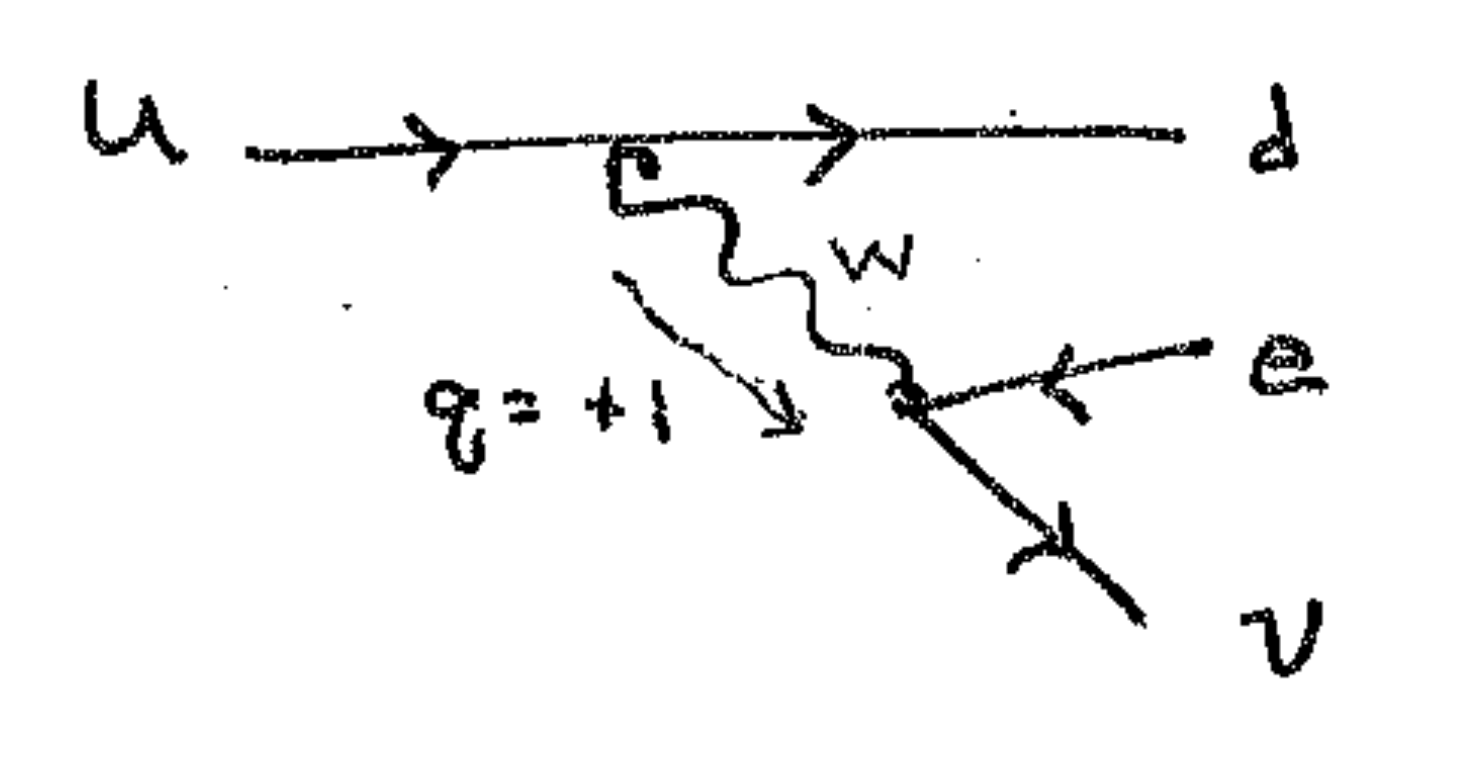
\includegraphics[width=.4\textwidth]{HW2b.png}
\end{center}
In this problem we will estimate the neutron lifetime and elucidate why our estimate in class was so wrong.

\subsubsection{Muon Lifetime}

We start with a slightly simpler example. Based on the above diagram, draw the diagram for $\mu \to \nu_\mu e \bar\nu_e$ . A useful fact: the amplitude for this diagram, $\mathcal A$, is approximately
\begin{align}
	\mathcal A = \left(\frac{g}{2\sqrt{2}}\right)^2 \frac{1}{M_W^2} \ .
\end{align}
Here $g/2\sqrt{2}$ is the strength of the interaction of the $W$ boson with a weak doublet\footnote{The factor of 2 is due to the fact that the $W$ boson only talks to left-handed particles. We will discuss this more in class. The factor of $\sqrt{2}$ is the same $\sqrt{2}$ in the normalization of $W^+ = (W^1 - iW^2)/\sqrt{2}$.}. Each vertex in the diagram comes with a factor of $g/2\sqrt{2}$, hence the diagram goes like the square of this factor. When the strength $g$ is increased, the value of the amplitude is increased. Makes sense. The factor of $M_W^{-2}$ encodes the internal $W$ boson line in the limit of low momentum transfer. As one increases $M_W$, the virtual $W$ becomes \emph{more} off-shell (more virtual), and the amplitudes decreases. 

The rate at which the muon decays is proportional to the square of the amplitude. $\Gamma \sim |\mathcal A|^2$. However, this doesn't have the correct dimensions for a rate. The remaining dimensions come from the characteristic energy scale of the system. Because the electron and neutrino masses are negligible, this mass scale has to be the muon mass, $m_\mu$. How many powers of the muon mass, $n$ are needed to write the rate?
\begin{align}
	\Gamma(\mu\to \nu_\mu e\bar\nu_e) = |\mathcal A|^2 (m_\mu)^n \ .
\end{align}

Write the order of magnitude of decay rate, $\Gamma$, in GeV using
\begin{align}
	g&\approx \frac{2}{3}
	&
	M_W &\approx 100~\text{GeV}
	&
	m_\mu &\approx 100~\text{MeV} \ .
\end{align}
Write the lifetime, $\tau = 1/\Gamma$, in seconds using $\hbar \approx \text{eV} \, \mu\text{s}$.




\subsubsection{Neutron Lifetime: wrong way}


Now perform the same analysis for the neutron lifetime by replacing $\mu$ with $u$. The relevant piece of information is that $m_u \approx 5~\text{MeV}$. This estimate, however, turns out to be wrong!

\subsubsection{Neutron lifetime: the correct way}

It turns out the above estimate is too na\"ive. The reason is that we neglected the mass of the final states. The positron and neutrino masses are still negligible compared to the up and down quark masses. However, the down quark is quite close to the up quark mass. We know that kinematically the rate must vanish if the down quark mass is increased to the up quark mass. Thus a better estimate for the rate is:
\begin{align}
	\Gamma = |\mathcal A|^2 \Delta m^n \ ,
\end{align}
where $\Delta m = m_u - m_d \approx \text{MeV}$ and $n$ is the power required for the right-hand side to have the dimensions of rate. What is the revised estimate for the neutron lifetime? 

My back of the envelope estimate is 100 seconds. This is about a factor of 1000 smaller than the na\"ive back of the envelope estimate where the down quark mass is neglected. Compare this to the actual neutron lifetime.

\textsc{Comment}: The suppression of the neutron decay is sometimes called `phase space' suppression. For muon decay, there are many different ways to assign momenta to the three on-shell final states while conserving four-momentum. Each of these contributes to the probability of the muon to decay. For neutron decay, there is much less \emph{phase space} to distribute four-momenta to the final states. 



% \subsection{Feedback}

% Approximately how long did it take you to complete the non-extra credit parts of this assignment?




\section{Extra Credit}

If you do any of these problems, please write a short note giving your thoughts on the reading: did you like them? Were they too simple / difficult? I do not expect you to be able to complete all (or necessarily any) of the extra credit.

\subsection{Direct Detection of Dark Matter}

This is an exercise in non-relativistic kinematics. One way to search for dark matter is to wait for it to hit a xenon nucleus and detect the recoil of the nucleus. In this problem, we use the `sum over all possible paths' mantra of quantum mechanics to explain why we use xenon as opposed to something cheaper, like helium. 

For simplicity, assume that both the mass of the dark matter and the mass of the xenon nucleus is $m_{\text{DM}} = m_{\text{Xe}}=100~$GeV. Assume that in the \textbf{lab frame}, the xenon nucleus is at rest and that the dark matter particle is traveling at $(v_\text{DM}^\text{lab})=300~$km/s. You can work to one significant figure in this problem (you may want to keep 2 significant figures for intermediate steps). 

\subsubsection{Momentum transfer}
The transfer 3-momentum, $\vec q$, is the 3-momentum that the incident dark matter particle imparts on the nucleus at rest. Everything is happening slowly enough that special relativity doesn't affect anything, so we can add velocities in the simple (Galilean) way. Derive the expression for the magnitude transfer momentum, 
\begin{align}
	|\vec q|^2 = 2\mu^2 (v_\text{DM}^\text{lab})^2 (1\pm \cos \theta_\text{cm}) \ ,
\end{align}
where the sign of the angle depends on how it's defined. Here `cm' means `center of mass frame', $\mu = m_{\text{DM}}m_{\text{Xe}}/(m_{\text{DM}}+m_{\text{Xe}})$ is the dark matter--nucleus reduced mass. This is an exercise in Newtonian kinematics.


\subsubsection{de Broglie wavelength}

\emph{You can do this independently of the previous part.} 

Estimate the magnitude of the momentum transfer,
\begin{align}
	|\vec q| \approx \mu (v_\text{DM}^\text{lab}) \ .
\end{align}
Recall that the \textbf{de Broglie wavelength} of a particle is $\lambda = 2\pi\hbar/|\vec q|$. Of course, $\hbar = 1$ in this class. What is the approximate de Broglie wavelength associated with the dark matter scattering off the nucleus?

This wavelength describes the length scale that the interaction is probing. The size of a `big' nucleus is around 10~fm. Confirm that the de Broglie wavelength encompasses a `big' nucleus.

\subsubsection{Coherent scattering}

We assume that dark matter interacts with the protons and neutrons in the nucleus. Protons and neutrons are collectively known as nucleons. We assume that the dark matter talks to all nucleons equally.
If the de Broglie wavelength is larger  than the size of the nucleus, then the dark matter particle `sees' all of nucleons in the nucleus. Thus if the dark matter scatters off the nucleus, the scattering is actually a sum over the amplitude for dark matter to scatter off of one of the protons, plus the amplitude for dark matter to scatter off of a different proton, plus the amplitude for dark matter to scatter off one of the neutrons, etc.

How much more \emph{likely} is it for dark matter to scatter off of a heavy nucleus with atomic mass number $A$ compared to a light nucleus like helium with atomic mass number 4? This is why we fill our detectors with liquid xenon rather than helium.




\end{document}